% Created 2023-02-01 Wed 18:04
\documentclass[9pt, b5paper]{article}
\usepackage{xeCJK}
\usepackage{minted}
\usepackage[T1]{fontenc}
\usepackage[scaled]{beraserif}
\usepackage[scaled]{berasans}
\usepackage[scaled]{beramono}
\usepackage{graphicx}
\usepackage{xcolor}
\usepackage{multirow}
\usepackage{multicol}
\usepackage{float}
\usepackage{textcomp}
\usepackage{algorithm}
\usepackage{algorithmic}
\usepackage{latexsym}
\usepackage{natbib}
\usepackage{geometry}
\geometry{left=1.2cm,right=1.2cm,top=1.5cm,bottom=1.2cm}
\newminted{common-lisp}{fontsize=\footnotesize} 
\usepackage[xetex,colorlinks=true,CJKbookmarks=true,linkcolor=blue,urlcolor=blue,menucolor=blue]{hyperref}
\author{deepwaterooo}
\date{\today}
\title{ET框架小游戏--斗地主源码学习}
\hypersetup{
  pdfkeywords={},
  pdfsubject={},
  pdfcreator={Emacs 27.2 (Org mode 8.2.7c)}}
\begin{document}

\maketitle
\tableofcontents


\section{几个项目,哪里先后是如何运行的?文件太多,傻傻分不清楚,可是一定会弄清楚的}
\label{sec-1}
\subsection{ETModel.Init.cs: 不可热更新,应该是它先起始,再启热更新层的启动文件}
\label{sec-1-1}
\begin{minted}[fontsize=\scriptsize,linenos=false]{csharp}
namespace ETModel {
    public class Init : MonoBehaviour {

        private async void Start() {
            try { 
                if (!Application.unityVersion.StartsWith("2017.4")) {
                    Log.Error($"新人请使用Unity2017.4版本,减少跑demo遇到的问题! 下载地址:\n https:// unity3d.com/cn/unity/qa/lts-releases?_ga=2.227583646.282345691.1536717255-1119432033.1499739574");
                }
                SynchronizationContext.SetSynchronizationContext(OneThreadSynchronizationContext.Instance); // 异步线程等的上下文自动同步
                DontDestroyOnLoad(gameObject);
                Game.EventSystem.Add(DLLType.Model, typeof(Init).Assembly); // Unity.Model 里面的代码不能热更新,通常将游戏中不会变动的部分放在这个项目里
                Game.Scene.AddComponent<GlobalConfigComponent>(); // 读取全局配置,不知道是否会触发什么回调
                Game.Scene.AddComponent<NetOuterComponent>();     // 客户端需要与登录服,网关服通消息,必须挂这个
                Game.Scene.AddComponent<ResourcesComponent>();
                Game.Scene.AddComponent<PlayerComponent>();
                Game.Scene.AddComponent<UnitComponent>();
                Game.Scene.AddComponent<UIComponent>();
                // 斗地主客户端自定义全局组件
                // 用于保存玩家本地数据
                Game.Scene.AddComponent<ClientComponent>();
                // 下载ab包
                await BundleHelper.DownloadBundle();
                Game.Hotfix.LoadHotfixAssembly();
                // 加载配置
                Game.Scene.GetComponent<ResourcesComponent>().LoadBundle("config.unity3d");
                Game.Scene.AddComponent<ConfigComponent>();
                Game.Scene.GetComponent<ResourcesComponent>().UnloadBundle("config.unity3d");
                Game.Scene.AddComponent<OpcodeTypeComponent>();
                Game.Scene.AddComponent<MessageDispatherComponent>();
                Game.Hotfix.GotoHotfix();
                Game.EventSystem.Run(EventIdType.TestHotfixSubscribMonoEvent, "TestHotfixSubscribMonoEvent");
            }
            catch (Exception e) {
                Log.Error(e);
            }
        }
        private void Update() {
            OneThreadSynchronizationContext.Instance.Update();
            Game.Hotfix.Update?.Invoke();
            Game.EventSystem.Update();
        }
        private void LateUpdate() {
            Game.Hotfix.LateUpdate?.Invoke();
            Game.EventSystem.LateUpdate();
        }
        private void OnApplicationQuit() {
            Game.Hotfix.OnApplicationQuit?.Invoke();
            Game.Close();
        }
    }
}
\end{minted}
\subsection{ETModel.Hotfix:}
\label{sec-1-2}
\begin{minted}[fontsize=\scriptsize,linenos=false]{csharp}
namespace ETModel {
    public sealed class Hotfix : Object {

#if ILRuntime
        private ILRuntime.Runtime.Enviorment.AppDomain appDomain;
#else
        private Assembly assembly;
#endif
        private IStaticMethod start;
        public Action Update;
        public Action LateUpdate;
        public Action OnApplicationQuit;

        public Hotfix() {
        }

        public void GotoHotfix() {
#if ILRuntime
            ILHelper.InitILRuntime(this.appDomain); // 这个方法里作:ILRuntime热更新的必要的加载
#endif
            // 在ETModel.Int中,加载Hotfix.dll的程序集,指定的开始函数为ETHotfix.Init.Start方法
            this.start.Run(); // <<<<<<<<<<<<<<<<<<<< 就是这些细节的地方,跟着跟着就会跟丢,要看下面的地方,有定义
        }

        public List<Type> GetHotfixTypes() {
#if ILRuntime
            if (this.appDomain == null) {
                return new List<Type>();
            }
            return this.appDomain.LoadedTypes.Values.Select(x => x.ReflectionType).ToList();
#else
            if (this.assembly == null) {
                return new List<Type>();
            }
            return this.assembly.GetTypes().ToList();
#endif
        }

        public void LoadHotfixAssembly() {
            Game.Scene.GetComponent<ResourcesComponent>().LoadBundle($"code.unity3d");
#if ILRuntime
            Log.Debug($"当前使用的是ILRuntime模式");
            this.appDomain = new ILRuntime.Runtime.Enviorment.AppDomain();
            GameObject code = (GameObject)Game.Scene.GetComponent<ResourcesComponent>().GetAsset("code.unity3d", "Code");
            byte[] assBytes = code.Get<TextAsset>("Hotfix.dll").bytes;
            byte[] mdbBytes = code.Get<TextAsset>("Hotfix.pdb").bytes;
            using (MemoryStream fs = new MemoryStream(assBytes))
                using (MemoryStream p = new MemoryStream(mdbBytes)) {
                    this.appDomain.LoadAssembly(fs, p, new Mono.Cecil.Pdb.PdbReaderProvider());
                }
            this.start = new ILStaticMethod(this.appDomain, "ETHotfix.Init", "Start", 0); // <<<<<<<<<< 这里说,起始方法是这么定义的
#else
            Log.Debug($"当前使用的是Mono模式");
            GameObject code = (GameObject)Game.Scene.GetComponent<ResourcesComponent>().GetAsset("code.unity3d", "Code");
            byte[] assBytes = code.Get<TextAsset>("Hotfix.dll").bytes;
            byte[] mdbBytes = code.Get<TextAsset>("Hotfix.mdb").bytes;
            this.assembly = Assembly.Load(assBytes, mdbBytes);
            Type hotfixInit = this.assembly.GetType("ETHotfix.Init");
            this.start = new MonoStaticMethod(hotfixInit, "Start");
#endif
            Game.Scene.GetComponent<ResourcesComponent>().UnloadBundle($"code.unity3d");
        }
    }
}
\end{minted}
\subsection{ETHotfix.Init.cs:这里就回到了热更新域里的起始配置点}
\label{sec-1-3}
\begin{minted}[fontsize=\scriptsize,linenos=false]{csharp}
namespace ETHotfix {
    public static class Init {

        public static void Start() {
            try {
#if ILRuntime
                if (!Define.IsILRuntime) {
                    Log.Error("mono层是mono模式, 但是Hotfix层是ILRuntime模式");
                }
#else
                if (Define.IsILRuntime) {
                    Log.Error("mono层是ILRuntime模式, Hotfix层是mono模式");
                }
#endif
                Game.Scene.ModelScene = ETModel.Game.Scene;
                // 注册热更层回调
                ETModel.Game.Hotfix.Update = () => { Update(); };
                ETModel.Game.Hotfix.LateUpdate = () => { LateUpdate(); };
                ETModel.Game.Hotfix.OnApplicationQuit = () => { OnApplicationQuit(); };
                
                Game.Scene.AddComponent<UIComponent>();
                Game.Scene.AddComponent<OpcodeTypeComponent>();
                Game.Scene.AddComponent<MessageDispatherComponent>();
                // 加载热更配置
                ETModel.Game.Scene.GetComponent<ResourcesComponent>().LoadBundle("config.unity3d");
                Game.Scene.AddComponent<ConfigComponent>();
                ETModel.Game.Scene.GetComponent<ResourcesComponent>().UnloadBundle("config.unity3d");
                UnitConfig unitConfig = (UnitConfig)Game.Scene.GetComponent<ConfigComponent>().Get(typeof(UnitConfig), 1001);
                Log.Debug($"config {JsonHelper.ToJson(unitConfig)}");
                // Game.EventSystem.Run(EventIdType.InitSceneStart);
                Game.EventSystem.Run(EventIdType.LandlordsInitSceneStart); // 这个特定事件是怎么运行的?不是标签系统吗,加载的时候已经扫过了,现在就是去跑这些扫过的标签方法
            }
            catch (Exception e) { 
                Log.Error(e);
            }
        }
        public static void Update() {
            try {
                Game.EventSystem.Update();
            }
            catch (Exception e) {
                Log.Error(e);
            }
        }
        public static void LateUpdate() {
            try {
                Game.EventSystem.LateUpdate();
            }
            catch (Exception e) {
                Log.Error(e);
            }
        }
        public static void OnApplicationQuit() {
            Game.Close();
        }
    }
}
\end{minted}
\subsection{ETHotfix.InitSceneStart\_CreateLandlordsLogin.cs}
\label{sec-1-4}
\begin{minted}[fontsize=\scriptsize,linenos=false]{csharp}
namespace ETHotfix {

 // 加载的时候,扫描到的标签系统,这个标签,就对应了这么个事件    
    [Event(EventIdType.LandlordsInitSceneStart)]
    public class InitSceneStart_CreateLandlordsLogin : AEvent {
        public override void Run() {
            // 创建登录界面
            UI ui = Game.Scene.GetComponent<UIComponent>().Create(UIType.LandlordsLogin);
        }
    }
}
\end{minted}

\section{服务器端的逻辑}
\label{sec-2}
\begin{itemize}
\item 感觉上面的客户端的起始逻辑大致还是能够理得清的
\item 这么无限地看下去,不知道到哪年哪月才能真正看得完,还是得赶快把自己的小服务器给弄起来
\item 那么就集中到自己想要实现的功能点:
\begin{itemize}
\item 一个热更新资源包的文件服务器,及下载文件的相关逻辑
\item 注册登录服:Realm
\item 网关服: Gate
\item DB服务器:用户信息,或更进一步的,游戏数据数据库服务器
\end{itemize}
\item 或者弄一个AllServer一个服务器解决一切问题,比较简单一点儿
\item 因为自己的服务器不是网络多人游戏,不涉及折到点儿的UI以及逻辑以及热更新的折分,只处理资源包文件服,登录登出拿取用户数据背个数据库,什么Map地图什么的全不涉及,应该能够简单狠多,可是现在大的框架把据不透,小的知识点还没能理解透,所以过程中应该还会有些曲折波折。
\item 所以现在今天晚上看服务器端的源码,试图着重把上面与自己关系更为重要的几个问题解决掉:哪些功能模块是必须的,哪些是可以砍砍杀杀砍掉的?
\item 现在看服务器客户端哪一端,都还感觉是盲人摸象,不知道是怎么回事,怎么才能够把具备(ET框架具备吗?)动态热更新能力的服务器端改造成只具备自己想要的功能的减小精悍的小小服务器(我的服务器可以不需要动态热更新能力。只需要我的客户端能够动态热更新资源包就可以了)?
\item 今天晚上把服务器端的源码理一理,就该试着用ET框架的framework来改造成自已的小小的服务器,完成自已游戏的最后最具挑战的部分了。
\end{itemize}
\subsection{框架的整体构总结理解}
\label{sec-2-1}
\subsection{客户端}
\label{sec-2-2}

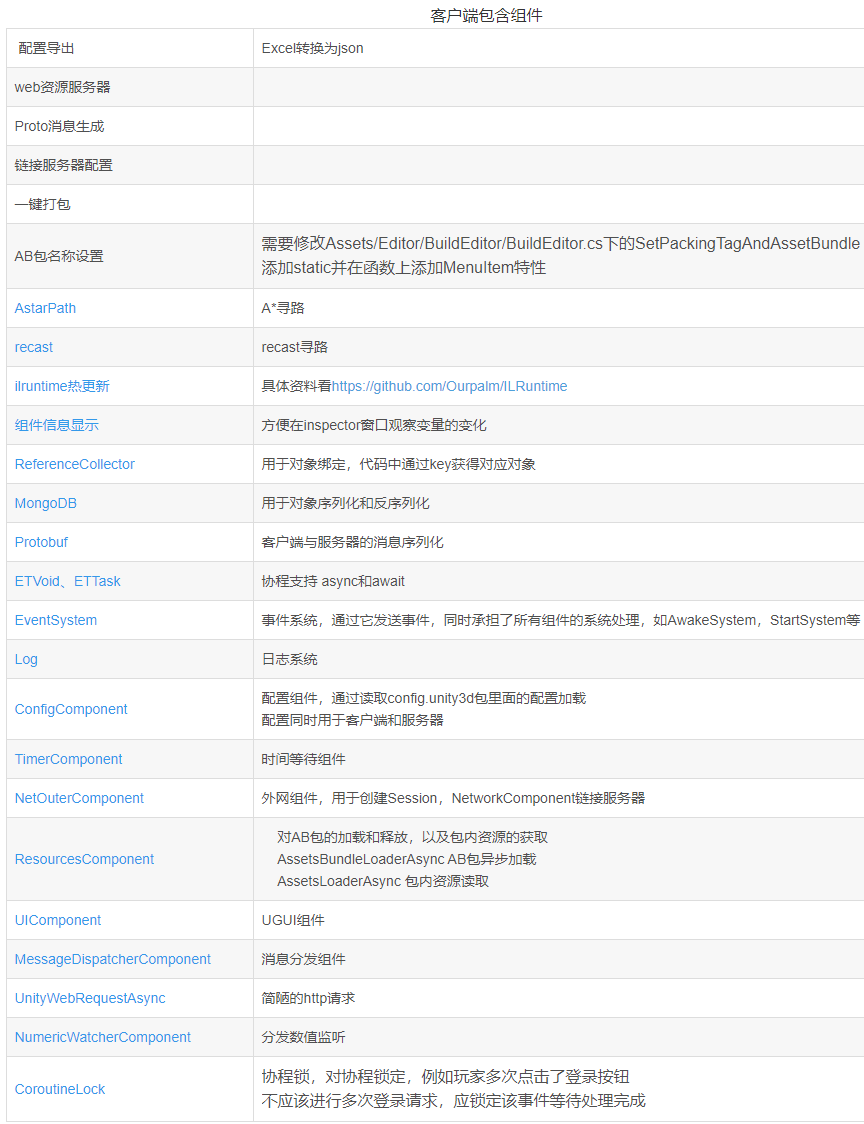
\includegraphics[width=.9\linewidth]{./pic/readme_20230131_220340.png}
\begin{center}
\begin{tabular}{lll}
\hline
配置导出 & Excel转换为json & \\
\hline
web资源服务器 &  & \\
Proto消息生成 &  & \\
链接服务器配置 &  & \\
一键打包 &  & \\
\hline
AB包名称设置 & 需要修改Assets/Editor/BuildEditor/BuildEditor.cs下的SetPackingTagAndAssetBundle & \\
 & 添加static并在函数上添加MenuItem特性 & \\
\hline
AstarPath & A*寻路: 这两个组件我的游戏中都不需要 & \\
recast & recast寻路 & \\
\hline
ilruntime热更新 & 具体资料看\url{https://github.com/Ourpalm/ILRuntime} & \\
组件信息显示 & 方便在inspector窗口观察变量的变化 & \\
ReferenceCollector & 用于对象绑定,代码中通过key获得对应对象 & \\
MongoDB & 用于对象序列化和反序列化 & \\
Protobuf & 客户端与服务器的消息序列化 & \\
\hline
ETVoid、ETTask & 协程支持 async和await & \\
EventSystem & 事件系统,通过它发送事件,同时承担了所有组件的系统处理,如AwakeSystem,StartSystem等 & \\
Log & 日志系统 & \\
ConfigComponent & 配置组件,通过读取config.unity3d包里面的配置加载 & \\
 & 配置同时用于客户端和服务器 & \\
TimerComponent & 时间等待组件 & \\
NetOuterComponent & 外网组件,用于创建Session,NetworkComponent链接服务器 & \\
\hline
ResourcesComponent & 对AB包的加载和释放,以及包内资源的获取 & \\
AssetsBundleLoaderAsync & AB包异步加载 & \\
AssetsLoaderAsync & 包内资源读取 & \\
\hline
UIComponent & UGUI组件 & \\
MessageDispatcherComponent & 消息分发组件 & \\
UnityWebRequestAsync & 简陋的http请求 & \\
NumericWatcherComponent & 分发数值监听 & \\
\hline
CoroutineLock & 协程锁,对协程锁定,例如玩家多次点击了登录按钮 & \\
 & 不应该进行多次登录请求,应锁定该事件等待处理完成 & \\
\hline
\end{tabular}
\end{center}
\subsection{服务器端的逻辑}
\label{sec-2-3}

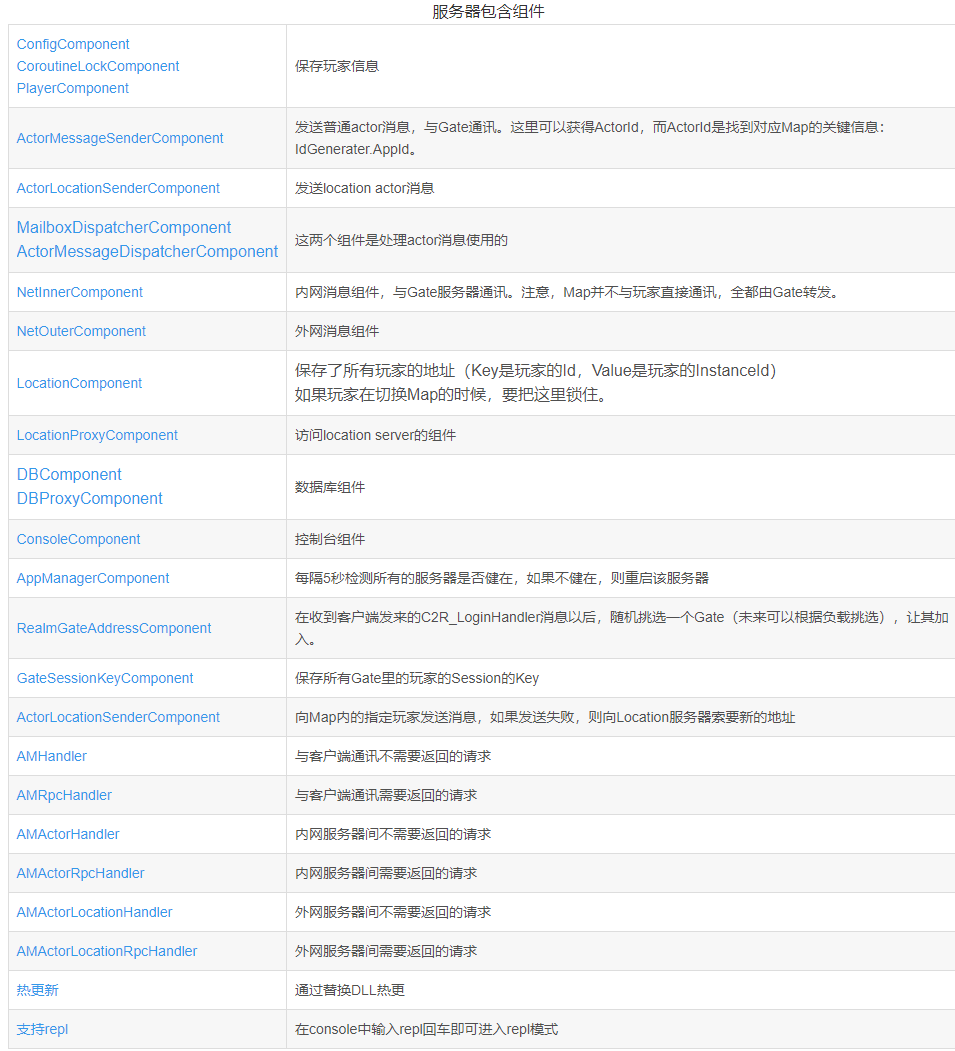
\includegraphics[width=.9\linewidth]{./pic/readme_20230131_221134.png}
\subsection{ET框架的Scene树}
\label{sec-2-4}
\begin{itemize}
\item 在ET框架下,Scene即为场景作为根节点,根节点下可以存放多个实体或组件。但Scenen本质也是实体,所以Scene之间也会有层次关系。
\item 游戏客户端的Scene层次结构
\end{itemize}

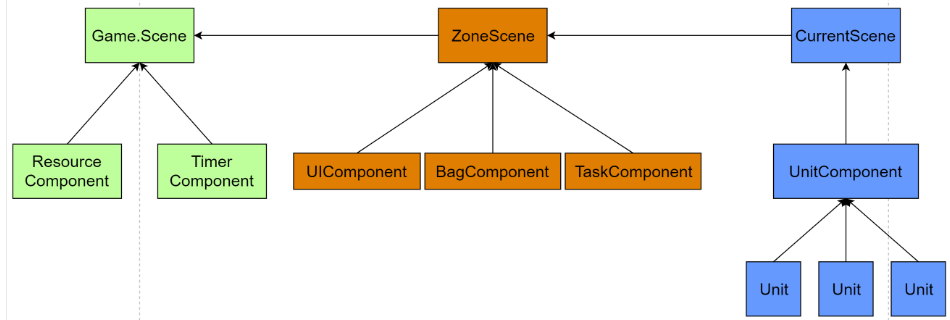
\includegraphics[width=.9\linewidth]{./pic/readme_20230201_122307.png}
\begin{itemize}
\item GameScene
\begin{itemize}
\item 游戏客户端全局的Scene根节点,用于提供游戏客户端全局且必要的基础功能组件(资源加载管理组件,计时器组件等)
\end{itemize}
\item ZoneScene
\begin{itemize}
\item 用于提供玩家全局游戏业务功能逻辑组件(例如基础UI,背包界面等)
\end{itemize}
\item CurrentScene
\begin{itemize}
\item 代表玩家当前所在的地图场景,一般用于挂载当前场景相关的组件,切换或释放场景时回收所有实体及组件。
\end{itemize}
\end{itemize}
\subsection{游戏服务端Scene层次结构}
\label{sec-2-5}

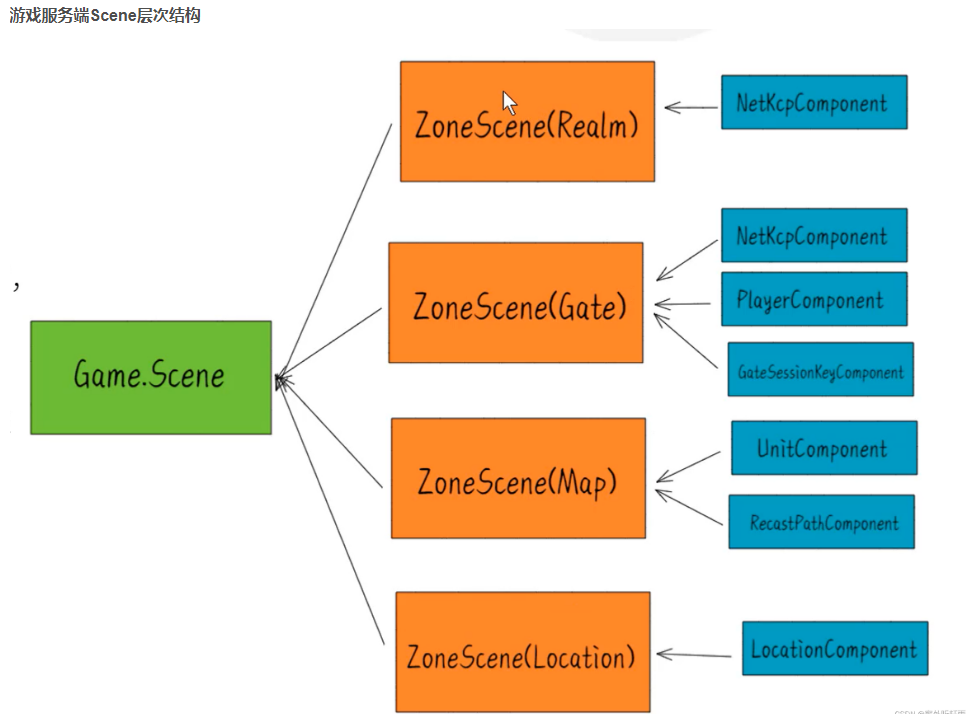
\includegraphics[width=.9\linewidth]{./pic/readme_20230201_141859.png}
\begin{itemize}
\item GameScene
\begin{itemize}
\item 类似客户端,其用来挂载全局服务端所需的基础功能必备组件
\end{itemize}
\item ZoneScene
\begin{itemize}
\item 可以创建多个不同功能的ZoneScene, 每个不同功能的ZoneScene下挂载其应该具有的功能组件,例如网关下的NetKcpComponent,定位服务器的LocationComponent等等,一般通过SceneType的枚举对其进行逻辑分发。
\item 不同ZoneScene可以存在一个进程上面,也可以每个都ZoneScene运行在一个单独的进程上,不同ZoneScene进程甚至可以分布在服务器集群上,大大提高了运行效率。
\item Scene可以动态创建和销毁(用于制作副本等临时场景)
\end{itemize}
\end{itemize}
\subsection{创建Scene的一般流程}
\label{sec-2-6}
\begin{itemize}
\item 创建一个未挂载任何组件的Scene对象 Scene scene = EntitySceneFactory.CreateScene(id, instanceId, zone, sceneType, name, parent);
\item 添加服务器下Scene的公共组件mailBox(用于接收Actor消息),scene.AddComponent<MailBoxComponent, MailboxType>(MailboxType.UnOrderMessageDispatcher);
\item 根据scene.SceneType针对不同服务器添加相应的组件,做相应的逻辑处理。
\end{itemize}
\begin{minted}[fontsize=\scriptsize,linenos=false]{csharp}
switch (scene.SceneType)
{
	case SceneType.Realm:
		scene.AddComponent<NetKcpComponent, IPEndPoint, int>(startSceneConfig.OuterIPPort, SessionStreamDispatcherType.SessionStreamDispatcherServerOuter);
		break;
 	case SceneType.Gate:
        scene.AddComponent<NetKcpComponent, IPEndPoint, int>(startSceneConfig.OuterIPPort, SessionStreamDispatcherType.SessionStreamDispatcherServerOuter);
        scene.AddComponent<PlayerComponent>();
        scene.AddComponent<GateSessionKeyComponent>();
        break;
   	case SceneType.Map:
        scene.AddComponent<UnitComponent>();
        scene.AddComponent<AOIManagerComponent>();
        break;
    case SceneType.Location:
        scene.AddComponent<LocationComponent>();
        break;
}
\end{minted}
\section{小小小小小服务器:要怎么才能开始动手试图去实现这个小服务器呢?}
\label{sec-3}
\subsection{如果适配ET框架,现游戏可能哪些模块版块存在问题}
\label{sec-3-1}
\begin{itemize}
\item 我也觉得ET框架可能不太适合我现在的游戏(也就是说,把我的游戏完全适配成ET框架来开发,原本只需要一个小小服务器,完全适配为ET框架,就把问题弄得狠复杂了。。。),
\item 使用ET框架,我所有的安卓基础就会被抛到九宵去外,不再关安卓SDK  NDK什么事儿了。。。。。是对自己太大的损耗。而我原本还可以简单封装实现的安卓录屏,游戏内使用安卓SDK相关功能模块录屏游戏过程等,会被全部废掉,损失太大不值得。我觉得我就只要个文件服务器加个数据库而已。
\item 原因是:我现在还想不通若是用ET框架来实现自己游戏的(服务器与客户端双端都可以热更新),我该如何实现我的方块砖10个按钮上的点击事件,射线检测?它的ILRuntime热更新程序域里对射线检测包的组件安装可能会成为自己狠大的问题,因为还不是狠懂里面的内部原理.这个模块重构的原理是:把射线检测,如果必要一定要,封装成如ET中任何其它可装载卸载的组件一样的装载到某个必要场景上去.ET里有个检测鼠标左右键位置的帮助类,但跟射线检测应该还是相差狠远的.
\item 所以,现在对这个框架,最深的感触是:盲人摸象,摸每部分细节似乎都快清楚了,却无法组装从一个更高的层面上来理解和把握框架设计,无法吃透,在大框架功能模块上犯难,在网上再搜一搜
\item 我可以把两组按钮画面同样做成预设与热更新资源包,射线检测同样会成为可装载可卸载的组件,可是再后面射线检测到的物体逻辑,感觉有点儿复杂了
\item 
\item 
\end{itemize}
\subsection{如果不适配,怎么弄个服务器带数据库等逻辑?}
\label{sec-3-2}
\begin{itemize}
\item 使用部分共享源码的双端(共享的是文件服务器8个项目,MongoDB数据库服务器, Realm注册登录用,网关服,Location服, ETTAsk, RPC消息机制, NetComponent等自己机对陌生需要练习,而自己的服务器也不可缺省的相关功能)
\item 现在知道自己整的不沦不类的服务器所谓的登录,登录的是网页上的认证相关,跟自己真正要实现的游戏里注册登录服保存数据库完全两回事,现在知道了。
\item 作用ET的头,实现用户注册与登录,适配自己现有游戏的尾,游戏除了入口之外全游戏进热更新程序域里
\item 那么自己的现框架架构作尾,全游戏逻辑进热更新域,存在的问题就变成是:
\item 我无法再实时动态检查用记上下线顶号之类的,我只能默认登录过就是登录状态,可是用户下线了,或更严格的说掉线了,服务器并不及时知道,可以通过安卓SDK中的按钮登出知道。但是掉网了掉线了呢?
\item 再则,ILRuntime热更新程序域里,我又该如何实现在热更新程序域里网络上载用户的游戏保存进展?这里需要去想和理解,为什么它ET框架就可以在热更新程序域里同网络交互,你哪里还没有想明白?
\item ET框架,热更新程序域里装载的组件,只是帮助与外界游戏程序域连通好,真正的网络请求上传下载等是在热更新域外面完成链接式传进去的?感觉对这个大框架没有掌握好,脑袋仍然是在像糊糊一样。。。
\item 各种泛型,接口的定义,一二三个参数等的泛型接口定义(你可以去找一找工程中的各种ILRuntime的适配器),全都是都可以成为热更新域里能够被游戏程序域里识别的原因,所以狠多设计,自带ILRuntime的适配性质
\item 去看热更新域里的适配初配置,可以看见它注册重定向了狠多函数签名的调用
\end{itemize}
\begin{minted}[fontsize=\scriptsize,linenos=false]{csharp}
namespace ETModel {
    public static class ILHelper {

        public static void InitILRuntime(ILRuntime.Runtime.Enviorment.AppDomain appdomain) {
            // 注册重定向函数
            // 注册委托
            appdomain.DelegateManager.RegisterMethodDelegate<List<object>>();
            appdomain.DelegateManager.RegisterMethodDelegate<AChannel, System.Net.Sockets.SocketError>();
            appdomain.DelegateManager.RegisterMethodDelegate<byte[], int, int>();
            appdomain.DelegateManager.RegisterMethodDelegate<IResponse>();
            appdomain.DelegateManager.RegisterMethodDelegate<Session, object>();
            appdomain.DelegateManager.RegisterMethodDelegate<Session, byte, ushort, MemoryStream>();
            appdomain.DelegateManager.RegisterMethodDelegate<Session>();
            appdomain.DelegateManager.RegisterMethodDelegate<ILTypeInstance>();
            appdomain.DelegateManager.RegisterFunctionDelegate<Google.Protobuf.Adapt_IMessage.Adaptor>();
            appdomain.DelegateManager.RegisterMethodDelegate<Google.Protobuf.Adapt_IMessage.Adaptor>();
            appdomain.DelegateManager.RegisterFunctionDelegate<Google.Protobuf.Adapt_IMessage.Adaptor, System.Boolean>();
            appdomain.DelegateManager.RegisterDelegateConvertor<System.Predicate<Google.Protobuf.Adapt_IMessage.Adaptor>>((act) => {
                return new System.Predicate<Google.Protobuf.Adapt_IMessage.Adaptor>((obj) => {
                    return ((Func<Google.Protobuf.Adapt_IMessage.Adaptor, System.Boolean>)act)(obj);
                });
            });
            CLRBindings.Initialize(appdomain);
            // 注册适配器
            Assembly assembly = typeof(Init).Assembly;
            foreach (Type type in assembly.GetTypes()) { // 程序集里还有些ILAdapter标标签可扫
                object[] attrs = type.GetCustomAttributes(typeof(ILAdapterAttribute), false);
                if (attrs.Length == 0) {
                    continue;
                }
                object obj = Activator.CreateInstance(type);
                CrossBindingAdaptor adaptor = obj as CrossBindingAdaptor;
                if (adaptor == null) {
                    continue;
                }
                appdomain.RegisterCrossBindingAdaptor(adaptor);
            }
            LitJson.JsonMapper.RegisterILRuntimeCLRRedirection(appdomain);
        }
    }
}
\end{minted}
\begin{itemize}
\item 举个标标签的例子:
\begin{minted}[fontsize=\scriptsize,linenos=false]{csharp}
namespace Google.Protobuf {

    [ILAdapter]
    public class Adapt_IMessage: CrossBindingAdaptor {
        public override Type BaseCLRType {
            get {
                return typeof (IMessage);
            }
        }
        public override Type AdaptorType {
            get {
                return typeof (Adaptor);
            }
        }
        public override object CreateCLRInstance(AppDomain appdomain, ILTypeInstance instance) {
            return new Adaptor(appdomain, instance);
        }

        public class Adaptor: MyAdaptor, IMessage {
            public Adaptor(AppDomain appdomain, ILTypeInstance instance): base(appdomain, instance) {
            }
            protected override AdaptHelper.AdaptMethod[] GetAdaptMethods() {
                AdaptHelper.AdaptMethod[] methods = {
                    new AdaptHelper.AdaptMethod { Name = "MergeFrom", ParamCount = 1 },
                    new AdaptHelper.AdaptMethod { Name = "WriteTo", ParamCount = 1 },
                    new AdaptHelper.AdaptMethod { Name = "CalculateSize", ParamCount = 0 },
                };
                return methods;
            }
            public void MergeFrom(CodedInputStream input) {
                Invoke(0, input);
            }
            public void WriteTo(CodedOutputStream output) {
                Invoke(1, output);
            }
            public int CalculateSize() {
                return (int) Invoke(2);
            }
        }
    }
}
\end{minted}
\item 那么就可以小一点儿一点儿地来,先弄个登录窗口,实现服务器的注册登录保存登录信息到数据库,相对比较小点儿的逻辑.这个过程中把MongoDB数据库的配置等所有连接过程中必要的步骤,可能出现的问题给解决掉,就算前进了一小步呀
\item 不知道怎么开始,也不知道怎么创建可以㠌套的像是安卓模块库一样的子工程,就只能把小游戏斗地主复制一份了再从它的基础上来改?!!!
\item 如果简单一点儿开始,我觉得我应该是可以先把简单点儿的MongoDB数据库连接成功,把用户登录相关的逻辑,网络交互的部分,ETTask RPC ACTOR消息等,哪怕是复制,把这部分弄过去
\end{itemize}
\subsection{点击注册后的日志(5  5)}
\label{sec-3-3}
\begin{minted}[fontsize=\scriptsize,linenos=false]{text}
(Program.cs:31) server start........................ 1 AllServer
{ "_t" : "C2R_Register_Req", "RpcId" : 1, "Account" : "5", "Password" : "5" }
{ "_t" : "DBQueryJsonRequest", "RpcId" : 1, "CollectionName" : "AccountInfo", "Json" : "{ \"Account\" : \"5\" }" }
{ "_t" : "DBQueryJsonRequest", "RpcId" : 1, "CollectionName" : "AccountInfo", "Json" : "{ \"Account\" : \"5\" }" }
{ "_t" : "DBQueryJsonResponse", "Components" : [], "RpcId" : 1, "Error" : 0, "Message" : null }
{ "_t" : "DBQueryJsonResponse", "Components" : [], "RpcId" : 1, "Error" : 0, "Message" : null }
(C2R_Register_ReqHandler.cs:32) 注册新账号:{ "_t" : "AccountInfo", "_id" : NumberLong("391266970697921"), "C" : [], "Account" : "5", "Password" : "5" }
{ "_t" : "DBSaveRequest", "RpcId" : 2, "NeedCache" : true, "CollectionName" : null, "Component" : { "_t" : "AccountInfo", "_id" : NumberLong("391266970697921"), "C" : [], "Account" : "5", "Password" : "5" } }
{ "_t" : "DBSaveRequest", "RpcId" : 2, "NeedCache" : true, "CollectionName" : null, "Component" : { "_t" : "AccountInfo", "_id" : NumberLong("391266970697921"), "C" : [], "Account" : "5", "Password" : "5" } }
{ "_t" : "DBSaveResponse", "RpcId" : 2, "Error" : 0, "Message" : null }
{ "_t" : "DBSaveResponse", "RpcId" : 2, "Error" : 0, "Message" : null }
{ "_t" : "DBSaveRequest", "RpcId" : 3, "NeedCache" : false, "CollectionName" : null, "Component" : { "_t" : "UserInfo", "_id" : NumberLong("391266970697921"), "C" : [], "NickName" : "用户5", "Wins" : 0, "Loses" : 0, "Money" : NumberLong(10000) } }
{ "_t" : "DBSaveRequest", "RpcId" : 3, "NeedCache" : false, "CollectionName" : null, "Component" : { "_t" : "UserInfo", "_id" : NumberLong("391266970697921"), "C" : [], "NickName" : "用户5", "Wins" : 0, "Loses" : 0, "Money" : NumberLong(10000) } }
{ "_t" : "DBSaveResponse", "RpcId" : 3, "Error" : 0, "Message" : null }
{ "_t" : "DBSaveResponse", "RpcId" : 3, "Error" : 0, "Message" : null }
{ "_t" : "R2C_Register_Ack", "RpcId" : 1, "Error" : 0, "Message" : "" }
{ "_t" : "C2R_Login_Req", "RpcId" : 2, "Account" : "5", "Password" : "5" }
(C2R_Login_ReqHandler.cs:14) 登录请求:{Account:'5',Password:'5'}
{ "_t" : "DBQueryJsonRequest", "RpcId" : 4, "CollectionName" : "AccountInfo", "Json" : "{ \"Account\" : \"5\", \"Password\" : \"5\" }" }
{ "_t" : "DBQueryJsonRequest", "RpcId" : 4, "CollectionName" : "AccountInfo", "Json" : "{ \"Account\" : \"5\", \"Password\" : \"5\" }" }
{ "_t" : "DBQueryJsonResponse", "Components" : [{ "_t" : "AccountInfo", "_id" : NumberLong("391266970697921"), "C" : [], "Account" : "5", "Password" : "5" }], "RpcId" : 4, "Error" : 0, "Message" : null }
{ "_t" : "DBQueryJsonResponse", "Components" : [{ "_t" : "AccountInfo", "_id" : NumberLong("391266970697921"), "C" : [], "Account" : "5", "Password" : "5" }], "RpcId" : 4, "Error" : 0, "Message" : null }
(C2R_Login_ReqHandler.cs:23) 账号登录成功{ "_t" : "AccountInfo", "_id" : NumberLong("391266970697921"), "C" : [], "Account" : "5", "Password" : "5" }
{ "_t" : "R2G_GetLoginKey_Req", "RpcId" : 5, "UserID" : NumberLong("391266970697921") }
{ "_t" : "R2G_GetLoginKey_Req", "RpcId" : 5, "UserID" : NumberLong("391266970697921") }
{ "_t" : "G2R_GetLoginKey_Ack", "RpcId" : 5, "Error" : 0, "Message" : null, "Key" : NumberLong("2874171809693671335") }
{ "_t" : "G2R_GetLoginKey_Ack", "RpcId" : 5, "Error" : 0, "Message" : null, "Key" : NumberLong("2874171809693671335") }
{ "_t" : "R2C_Login_Ack", "RpcId" : 2, "Error" : 0, "Message" : "", "Key" : NumberLong("2874171809693671335"), "Address" : "127.0.0.1:10002" }
{ "_t" : "C2G_LoginGate_Req", "RpcId" : 3, "Key" : NumberLong("2874171809693671335") }
{ "_t" : "ObjectAddRequest", "RpcId" : 6, "Key" : NumberLong("391266970697944"), "InstanceId" : NumberLong("391266970697944") }
{ "_t" : "ObjectAddRequest", "RpcId" : 6, "Key" : NumberLong("391266970697944"), "InstanceId" : NumberLong("391266970697944") }
(LocationComponent.cs:64) location add key: 391266970697944 instanceId: 391266970697944
{ "_t" : "ObjectAddResponse", "RpcId" : 6, "Error" : 0, "Message" : null }
{ "_t" : "ObjectAddResponse", "RpcId" : 6, "Error" : 0, "Message" : null }
{ "_t" : "ObjectAddRequest", "RpcId" : 7, "Key" : NumberLong("391266970697942"), "InstanceId" : NumberLong("391266970697942") }
{ "_t" : "ObjectAddRequest", "RpcId" : 7, "Key" : NumberLong("391266970697942"), "InstanceId" : NumberLong("391266970697942") }
(LocationComponent.cs:64) location add key: 391266970697942 instanceId: 391266970697942
{ "_t" : "ObjectAddResponse", "RpcId" : 7, "Error" : 0, "Message" : null }
{ "_t" : "ObjectAddResponse", "RpcId" : 7, "Error" : 0, "Message" : null }
{ "_t" : "G2R_PlayerOnline_Req", "RpcId" : 8, "UserID" : NumberLong("391266970697921"), "GateAppID" : 1 }
{ "_t" : "G2R_PlayerOnline_Req", "RpcId" : 8, "UserID" : NumberLong("391266970697921"), "GateAppID" : 1 }
(G2R_PlayerOnline_ReqHandler.cs:21) 玩家391266970697921上线
{ "_t" : "R2G_PlayerOnline_Ack", "RpcId" : 8, "Error" : 0, "Message" : null }
{ "_t" : "R2G_PlayerOnline_Ack", "RpcId" : 8, "Error" : 0, "Message" : null }
{ "_t" : "G2C_LoginGate_Ack", "RpcId" : 3, "Error" : 0, "Message" : "", "PlayerID" : NumberLong("391266970697944"), "UserID" : NumberLong("391266970697921") }
{ "_t" : "C2G_GetUserInfo_Req", "RpcId" : 4, "UserID" : NumberLong("391266970697921") }
{ "_t" : "DBQueryRequest", "RpcId" : 9, "_id" : NumberLong("391266970697921"), "CollectionName" : "UserInfo", "NeedCache" : false }
{ "_t" : "DBQueryRequest", "RpcId" : 9, "_id" : NumberLong("391266970697921"), "CollectionName" : "UserInfo", "NeedCache" : false }
{ "_t" : "DBQueryResponse", "RpcId" : 9, "Error" : 0, "Message" : null, "Component" : { "_t" : "UserInfo", "_id" : NumberLong("391266970697921"), "C" : [], "NickName" : "用户5", "Wins" : 0, "Loses" : 0, "Money" : NumberLong(10000) } }
{ "_t" : "DBQueryResponse", "RpcId" : 9, "Error" : 0, "Message" : null, "Component" : { "_t" : "UserInfo", "_id" : NumberLong("391266970697921"), "C" : [], "NickName" : "用户5", "Wins" : 0, "Loses" : 0, "Money" : NumberLong(10000) } }
{ "_t" : "G2C_GetUserInfo_Ack", "RpcId" : 4, "Error" : 0, "Message" : "", "NickName" : "用户5", "Wins" : 0, "Loses" : 0, "Money" : NumberLong(10000) }
\end{minted}
% Emacs 27.2 (Org mode 8.2.7c)
\end{document}